
%
% Chapter 1
%

\chapter{INTRODUCTION}

\section{Motivation}
The development and application of wireless technology in the past few years has been astonishing. In the coming years, access to spectrum will be an increasingly important foundation for America's economic growth and technological leadership \cite{PCASTSpectrumReport2013}. The current process of long-term static frequency allocation cannot meet such demand, and the inefficient use in some parts of the spectrum by current wireless devices has led to significant research activities in cognitive radio (CR) and dynamic spectrum access (DSA) \cite{LeeAndHaenggi2012}, \cite{ QingZhaoandBMSadler2007}. The definition for Cognitive Radio has been evolving since 1999 \cite{IMitolaJandJMaguire1999}. The Federal Communications Commission (FCC) defines cognitive radio as a ``radio or system that senses its operational electromagnetic environment and can dynamically and autonomously adjust its radio operating parameters to modify system operation, such as maximize throughput, mitigate interference, facilitate interoperability, or access secondary markets'' \cite{FederalCommunicationsCommission:2005}. A main component of cognitive radio is DSA.

Much of the research on CR and DSA focuses on a priority-based approach in which radios are classified into two types of users called primary users and secondary users. Primary users have high priority or legacy rights for the usage of a specific part of the spectrum. Secondary users can access the spectrum as long as they do not cause harmful interference to the primary users \cite{GoldsmithANDJafarANDMaric2009}.

There have been some standards for priority-based dynamic spectrum sharing such as the IEEE 802.22 TV White Space Standard and the IEEE 802.11af Standard. The FCC and the National Telecommunications and Information Administration (NTIA) are developing a protocol that may allow devices with small cell technology to use the 3550-3650 MHz radar band \cite{Strickling2012}.

However, if there are multiple wireless systems without a pre-established priority trying to share the same spectrum, the spectrum sharing algorithms based on priority  may not be as efficient. Consequently, algorithms for distributed spectrum access as shown in Figure~\ref{fig:motivationExampleDSA}need to be explored.

\begin{figure}[tpb]
  \begin{center}
    \centerline{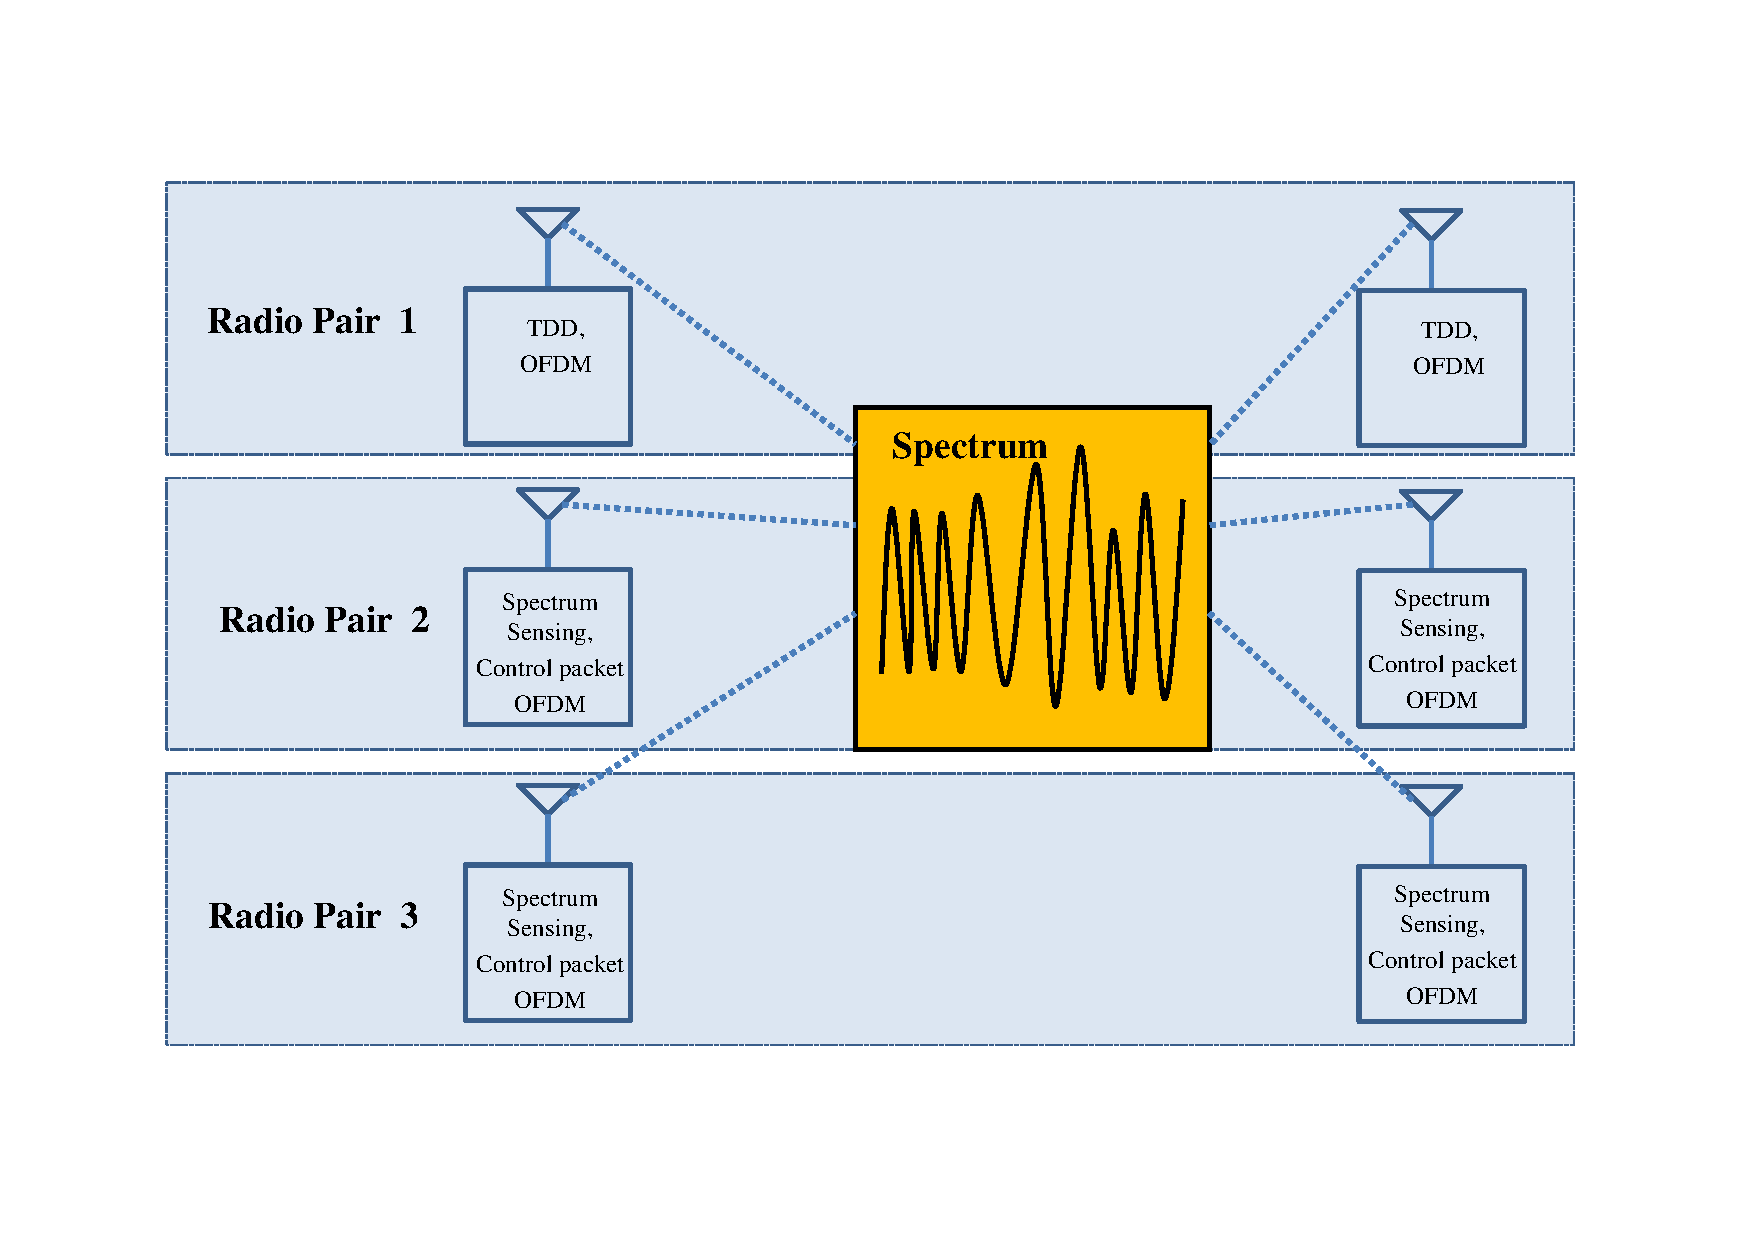
\includegraphics[width=160mm]{motivationExampleDSA.pdf}}
    \caption{Illustration of a distributed spectrum access system in which different types of radios try to share the same spectrum.}
    \label{fig:motivationExampleDSA}
  \end{center}
\end{figure}


This thesis focuses on both cooperative and competitive distributed spectrum access. In a cooperative distributed spectrum access system, standardized handshaking signals among all users could be used to achieve synchronization, depending on the application. For example, one user can claim to use part of the spectrum for a certain period of time by broadcasting an occupying or beacon signal, and all other users would avoid the spectrum occupied by the beacon signal and try to claim the right of another part of the spectrum. In this case, there should be a rule to enforce fair sharing of the spectrum. Otherwise, some greedy or malicious users can occupy the spectrum indefinitely. In other cases, handshaking signals are not used. For example, under severe conditions or extreme situations, such as natural disasters or accidents, it is desirable to have radios that can effectively and efficiently share the spectrum without direct coordination or spectrum preplanning. The FCC has designated a 700 MHz (698-806 MHz) frequency band for emergency use \cite{LLuYLi2012}.

In a competitive distributed spectrum access system, two or more users try to utilize the spectrum as much as possible. At the same time, each user interferes with other users, requiring robust signaling formats and often lower effective data rates and lower spectral efficiency. The objective of maximizing one��s own throughput and the objective of minimizing the throughput of competitors are usually consistent with each other. For instance, maximizing the transmission signal power has the potential not only to increase its own throughout but also to decrease competitors' throughout.

There is usually a power constraint for each user. Algorithms on the distribution of power across the spectrum need to be explored in terms of information theory and practical applications. There is a big gap between the information theory and the practical applications when developing power assignment algorithms. For example, in information theory, power can be assigned arbitrarily across frequency, but power assignment in practical application is limited by many factors, such as power amplifiers and modulation methods.

The Defense Advanced Research Projects Agency (DARPA) has initialized a program called the DARPA Spectrum Challenge to seek robust communications in a communication channel with unknown interfering signals \cite{DARPASpectrumChallenge}. The DARPA Spectrum Challenge consists of a cooperative competition and a competitive competition. The cooperative competition is a case of cooperative distributed spectrum access without standardized handshaking signal. The competitive competition is a case of competitive distributed spectrum access. In both competitions, each user has no prior knowledge of the other users.

\section{Scope and Contributions}
This thesis is motivated by the DARPA Spectrum Challenge. Theoretical analysis is conducted, and practical radios are designed and implemented with the GNU Radio software and the Ettus Universal Software Radio Peripheral (USRP) hardware. The radio design is subject to the constraints of the DARPA Spectrum Challenge.

The primary contribution of this thesis is to design and implement both a cooperative and a competitive radio for the DARPA Spectrum Challenge. The rules are analyzed, and strategies for both cooperative and competitive radio are developed. For both cooperative and competitive radios, a feedback scheme is analyzed based on the opportunities and limitation of the games, and a packet management system is implemented. For the cooperative radio, we developed a spectrum sensing technique based on statistics of the received energy across frequency. For the competitive radio, a time division duplex (TDD) system is developed. Many of these system components are likely to be useful beyond the DARPA Spectrum Challenge.

This thesis is organized as follows. Chapter \ref{chap:backgound} summarizes background on experimental wireless research using software-defined radio (SDR) as well as distributed spectrum access. Chapter \ref{chap:strategy} introduces the strategies for both competitive and cooperative matches, and Chapter \ref{chap:strategyAnalysis} analyzes the competitive and cooperative feedback strategies based on the rules. In Chapter \ref{chap:spectrumAnalysis}, a software spectrum sensor is designed. Chapter \ref{chap:TDD} introduces the design and implementation of a TDD system for the competitive radio. Chapter \ref{chap:performance} shows the test results and finally the conclusions and future work are summarized in Chapter \ref{chap:conclusion}.

